\chapter{Mobile social networking}\label{chap1}


% ====SECTION 1 ================================================================
\section{Introduction}

Mobile devices have become a staple of our society, with everyone of
us owning at least one. They are everywhere and play increasingly greater roles
in the lives of most everyone. Their availability is rapidly spreading
throughout the world and making significant improvements in many lives. Mobile
technology is making our lives better than ever before. We are now able to be in
touch with those we need to reach no matter where we are.

Mobile technology makes possible documents transfer almost anywhere in
the world in small amount of time so business is addressed when it
encounters an emergency. It keeps employees and business owners connected
regardless of their position on the globe and increases the company
productivity. It also keeps the customer updated with information about services
they use. Mobile technology transformed how companies do business.

The daily uses of mobile technology have transformed us into a society tightly
connected to each other. We have friends through such connections, even though
we may have never met them in persons. Media became subject of discussion, never
possible before making the resultant friendships as strong as those in real
life.

 
We have more information in our hand than ever before. It has become easy and
natural for someone to quickly look up helpful resources for whatever activity
we need to do. Mobile application can even anticipate what information we need
and present it to us when it is most useful.


\section{Social mobile applications}

Increasing mobile Internet use has made information sharing experiences very
popular among the users. There are many type of services on which the content is
being shared. The most popular is the social network Facebook, which enables you
to share photos and personal content with your friends. Another one is Twitter
which enables you to share information in something similar with a blog.
The evolution of location-aware mobile technology has influenced the mobile
application industry offering users a more contextual experience. The Facebook
Messenger provides the users with the location of their communication partner
and the latest feature of Nearby Friends notifies the user whether a friend is
in the nearby location. The best examples are Google Maps and Google Earth whose
purpose is to store data and display the geographic proximity based on the
position of the user.

\section{Inter-Vehicle Communication}

Vehicle-to-vehicle wireless communication have emerged from the desire to
provide more safety, entertainment and comfortable driving to a huge number of
individuals that use vehicles on the roads every day.

It is a known fact that many car manufacturers have already introduced wireless
communication equipment in their cars. Volvo implementation is called ``Volvo on
Call'' \citep{volvo} and BMW implementation is called ``BMW Assist''
\cite{bmw_assist}. Their purpose is to help drivers in case of accidents or
collisions. Their current implementation use ``central'' infrastructure based
services based on cell phone technology, existing base stations, long range and
centralised servers. Naturally, the next step would be to modify the equipment
in order to provide Inter-Vehicle Communication.

Inter-vehicle Communication is a type of ad-hoc network which mainly uses
broadcast as a method of information distribution. The only limitations vehicles
may have are the available transmission capacity which depends on the rate and
the size of the information broadcasted.

As we mentioned, communication between vehicles means adding some benefits to
driving experience. Some of relevant information for sharing might be: accident
warnings, driving conditions, weather, announcements and even advertisements
with audio/video content. They provide useful information related to a limited
geographical area, for a limited amount of time. For example, an accident
happened a day ago would not be of much interest for the drivers, so the need of
limiting the life of information is obvious. The biggest challenge is making
the information ``float'', thus we try to analyze and test a communication
protocol further in this thesis.

\section{Weaknesses of network-based mobile application}
While social network applications are dependent on the infrastructure services
in order to overcome distances and to connect people around the world, relying
on the infrastructure services for location-aware application may introduce
issues regarding content and location relevance and security
~\cite{percomfloatingcontent}:
\begin{itemize}
\item {\it Location privacy} concerns may arise from the need of the application
to provide the user with the exact location, especially for the navigation
services like Google Maps or Waze. It needs determining it with a high level of
accuracy in order to obtain the right context information.
\item {\it Content privacy} issues occur because the shared information is
stored by a private company in a private ``central'' location and can be easily
subject to censorship.
\item {\it Connectivity} to the infrastructure services can be a problem,
especially for traveling users who may have to deal with high roaming charges, 
unavailability of data services, or no network coverage at all.
\item {\it Geographic validity} concerns the location characteristics of the
information. Locally relevant shared content may be of little interest to the
rest of the world, so storing it in an accessible location may only cause memory
waste.
\item {\it Temporal validity} concerns the temporal characteristics of the
information. Shared content which is stored in a ``central'' location is only
valid for a limited amount of time and it is rarely associated with an expiry
information. This practice leads to content never being deleted or never being
read either,thus wasting databases memory.
\item {\it User identification} of some kind is used usually in order to limit
the amount of data being shared which creates some sense of responsibility
towards the service provider. It can also be a privacy problem because the
information shared is associated with the owner and nowadays companies like
Facebook or Google are giving access to the records to security agencies for
population surveillance (most recent case being PRISM) or for marketing
purposes.
\end{itemize}

The solution to all the above problems is a content sharing service which is
entirely dependent on mobile devices in the vicinity using principles of
opportunistic networking. Bringing social media and content sharing into ad-hoc
networks seems it is the next frontier in mobile industry. It can be seen as an
extension to the Internet infrastructure, by bringing connectivity where the
infrastructure is not able to.




% ==== Floating Content (CHAPTER 2) ================================================

\chapter{Floating Content} \label{chap2}


This chapter will describe the Floating Content model of the data storage.
My application is based on this model used to simulate and observe the existence
behaviour of the content on a real world map. The analysis is presented in
detail in a further chapter.

\section{Introduction}
Floating Content network is a particular type of network that uses intermittent
connectivity also known as delay tolerant networks (DTN). Recently, the new term
disruption-tolerant networking has gained popularity in the United States.
Among the events that may generate disruption we can identify limits of wireless
radio range, noise, energy resources and sparsity of mobile nodes
\cite{wikipedia_dtn}. This concept of information sharing matches the needs of
context-aware applications because it keeps the spatial proximity in a close
relation with connectivity.

Context awareness is a characteristic of a mobile devices and includes different
types such as : identity, activity, time, and the most important for our
analysis, location. The application can determine what activities may occur near
the entity, the objects and people that are nearby.

A use case scenario of context-aware application could be a tourist guide
information sharing. When you're visiting an unfamiliar location, having an
application that provides you with information about the surroundings can be a
blessing. The content can include information, history about places you are
visiting, hotel and restaurants and their service quality, directions you have
to follow to reach a desired place and much more.

\section{Applications for Floating Content}

The features of floating content offer the user exciting opportunities but can
also offer some important difficulties. The most useful opportunity enables
localized information sharing without using infrastructure services and without
central data records. Since there is no remote access, it gives the user some
degree of privacy, as he must be present in order to ``see'' something which is
a usual concept in the daily life. The major challenge is that the
communications service makes no guarantees that the data will stay around until
its lifetime expires. For example, during the night the content is expected to
disappear. We can make intuitive deductions, which are assisted by the
simulations which will be later discussed. If the service is used in an
overcrowded place like a market square or a heavy traffic road, there is a high
probability that the content will float for some time, even if not all other
people use context-aware mobile devices. In the end, any type of
communication (event the best-effort) may be better than no communication at
all.

People's daily activities cause density fluctuations over the day which may be a
problem for the residing information in certain places. Thus, the information is
expected to remain available for no more than a few hours. Making predictions
that there will be enough people in that location is very limited for now.
However, a limited amount of time, let's say one hour of ``floating'' may be
enough for the application to do its job. As a solution, a user can be a
permanent seed, staying around and resending out updated content.

Multiple use cases can emerge from the floating content concept. One of them can
use infrastructure-less local data availability for advertising or selling
goods. This type of market could have a dynamic catalog of available
merchandise, being able to operate updates on the fly.

Another one is information sharing between tourists and visitors about the local
attractions or notifications about good services a certain hotel is offering.
Spreading news and keeping it localized, time-bounded and most important
anonymous can be another use case of floating content for which best-effort
operation perfectly suits the needs.

Overall, floating content can be used in many ways, taking into consideration
two important aspects of it. First, floating information is localized by design
so the developers should consider multiple data-oriented architecture.
The second aspect is that the concept is best effort, a problem which
the Internet infrastructure solves with repair mechanisms that can recover lost
packets. In our case, data that expires is irrecoverable in an area. Taking
these into account for future application will produce more interesting use
cases.

\section{Service model}

This section describes the floating content design and the environment
constraints that the architecture needs in order to work. We assume users to be
mobile nodes who are interested in the content generated by all other nodes. We
assume that they are using mobile devices with unlimited data memory in order to
handle the amount of data exchanged during their participation in ad-hoc
network. Also, there is no supporting infrastructure for the system.

We assume that nodes are uniformly distributed and travel independently, with a
constant speed. In \cite{uniform_distribution} it is shown that this mobility
model preserve the spatial node distribution at all time points.

The devices are equipped with wireless interfaces (Bluetooth or WLAN) to enhance
network communication. Analysis of performance for 802.11p standard displayed in
\cite {performance80211} have shown that using a bitrate of 6Mbps and a
payload of 500 bytes yields a delivery rate of up to 80\%. This indicates the
acceptable reliability and performance of IEEE 802.11p and confirms the
viability of floating up to several megabytes of data (from text messages to
photos). This standard is used also in our simulation which will be discussed in
a further chapter. Making intuitive judgements, we can determine that contacts
cannot last more than several tens of seconds, in vehicle case even less due to
their high speeds. Thus there will be no need for the mobile devices to reserve
a considerable amount of storage for the floating content.

The devices also need to be equipped with accurate systems which determine their
position, e.g. using GPS tracking, cellular base stations, cell tower
triangulations using WLAN access points or Wi-fi tracking which is a very
popular technology. Each of these methodologies has its own advantages which
will make them more appropriate in different domains regarding the facts like
accuracy percentage needed, battery consumption etc. but in order to provide the
best location based service, you need to acquire the most accurate location
coordinates. Finally, nodes need to synchronize their clock time to tag the
floating information; it can be done with the help of GPS or cellular networks.

When producing information, the application must tag the information with its
geographic origin, validity range and and time-to-live (TTL).
Other nodes decide if they store the information and will replicate it further
if they are in the associated anchor zone to others. The information is
explicitly allowed to disappear providing no guarantees about its availability.
If the lifetime of the content expires, it will be discarded by the application.
In consequence an item may disappear if there are no nodes (or to few) to
replicate it in its associated anchor zone, unless the creator is there to
re-issue it again.

\subsection{System operation}

As \cite{percomfloatingcontent} presents, a node generates information $I$ which
has a size of $s(I)$ and a defined lifetime (TTL). The information is tagged
with the anchor zone also which is defined by its geo-located center $P$ and two
radii: {\it r} identifies the {\it replication range}, inside which nodes
replicate the information to other nodes they meet on their way and {\it a}
defines the {\it availability range} inside which the information is still
stored with limited probability. As shown in the ~\ref{fig:anchor_zone} outside
the availability zone there exist no copy of the item in the node data storage.

\begin{figure}[bt]
 \centering
 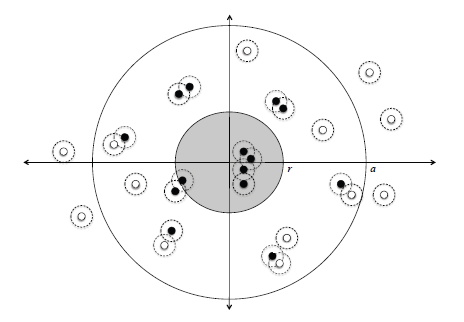
\includegraphics[width=0.6\textwidth]{img/anchor_zone}
 \caption{Moving nodes inside across an anchor zone. Black nodes are
 information-carrying nodes, white nodes will eventually get the information
 from the black ones. The probability of a node carrying an item tends to 1
 inside the replication zone, and decreases until reaching an availability a
 after which no more copies are found. }
 \label{fig:anchor_zone}
\end{figure}

The idea of the concept is that if two nodes meet in the anchor zone of some
information, and one of them doesn't have it stored in the data storage then the
other node will immediately send it so both nodes can be able to access it. As a
result, every node inside the anchor zone should have a copy of the item while
nodes which are leaving the anchor can delete it at their own discretion.

Let's consider two nodes A and B which encounter at some point in time. Node A
does have an item I tagged with an anchor zone centered in point P and radii
{\it a} and {\it r}. Let {\it h} be the distance of node A from the center P.
When node A meets node B, item I gets replicated to B with the probability
$p_r(h)$:

$$p_r(h) = \begin{cases}
	1 & \text{if } h \leq r \\
	R\left(h\right) & \text{if } r < h \leq a \\
	0 & \text{otherwise} \\
\end{cases}$$

$R(h)$ is a decreasing function which determines the probability of replication
between the outer replication border and the availability border of the anchor
zone.
The deletion probability $p_d(h)$ is defined as with $D(h)$ in $[0, 1]$ :

$$p_d(h) = \begin{cases}
	0 & \text{if } h \leq r \\
	D\left(h\right) & \text{if } r < h \leq a \\
	1 & \text{otherwise} \\
\end{cases}$$

The node preserves the free space due to the deletion function. It follows the
first in, first out (FIFO) principle, deleting the oldest items first if there
is a need for free space.

The area between {\it replication range} and {\it availability range} acts as a
buffer zone, that prevents immediate deletion of items. It is beneficial
for nodes that leave the {\it replication range} for a short period of time,
preventing them performing deletion operation. Thus, after returning inside
{\it replication range}, they have the associated items preserved. Outside the
anchor zone, a node could delete specific items when meeting with other nodes,
or at a predefined timeout, checking if items are outside their zones or their
lifetime expired.

As \cite{percomfloatingcontent} did, for simplicity and more trackability, in
our evaluation there is no buffer zone, i.e. {\it r = a}, deletion and replication
function becoming useless in this case.

\subsection{Communication Protocol}

As described in \cite{percomfloatingcontent}, the floating content protocol,
also used in our evaluations, is an efficient and simple method to exchange
items between nodes. A message is identified by a message id $Id$, the anchor point
with the attributes described earlier $(P,\ r,\ a)$, and the lifetime $T$. The
header of the message is filled with these characteristics, and the message body
of size $s(I)$ is filled with the desired payload.

Below is the protocol which has 4 phases:

\begin{enumerate}[1.]
  \item Nodes keep sending neighbor discovery beacons to discover peers.
  \item When receiving a discovery beacon, the peer decides to send in return,
  its list of items that verifies the condition $p_r(h) > 0$, thus valid for
  replication. In this phase the list contains only the attributes of the items,
  keeping this message as compact as possible: $Id$, $s(I)$, $(P, r, a)$ and
  lifetime $T$. If the list doesn't fit into a single message, it will be spread
  across multiple summary messages in a round-robin fashion.
  \item When receiving the list of items from a discovered peer, the node
  request those items for which $p_r(h)$ suggests that they should be replicated.
  \item In the last phase, requested items are exchanged until transfer
  completion or nodes lose contact. Upon this step, the protocol should remove
  uncompleted messages and return to phase 2.
\end{enumerate}

It is assumed that nodes can exchange messages fully bidirectional during any
step. Moreover, they can exchange messages simultaneously to multiple nodes
(even though technology may be limited). The beaconing process can take place
while in middle of message exchange in order to keep the discovering process
running. Since message exchanging is done in an incremental way, nodes can
append the new coming messages to the list, while they are still in transfer.

Deletion of item $I$ occurs immediately the node moves outside of $a$. In
\cite{percomfloatingcontent} is is suggested that a second possibility could be
deletion $upon-encounter$ which discards a message when meeting a new node.
stating that this policy is more sensible due to its asynchronous
characteristic triggered by an external event. Naturally, deletion takes place
before the list of items is sent to other peers.

\subsection{Security issues and resource management}

The presented protocol does not restrict the user in any way, regarding content
generation and its context parameters. The single requirement is that the owner
must be in the anchor zone at the time of creation. In consequence, this may
represent a flaw in the protocol, users being able to insert items in network
with an infinite anchor zone. Flooding items represent a threat for the network,
because they exhaust the system resources very quickly, especially channel and
buffer capacity.

Reputation mechanisms like \cite{reputation} or accounting could represent
solutions to the above spamming issues. But it would be very difficult to
implement them without having an central infrastructure to enhance
authentication of identities. Also being a best-effort service is another nail
in the coffin for the rewarding system. Some simple mechanisms could be added to
implementation like prioritizing items taking into consideration their expected
storage consumption and the distance from the anchor. Thus, deleting the
farthest or the most largest item may discourage unlimited content distribution.

As shown in \cite{percomfloatingcontent}, the application can smartly manage its
resources by giving preference to items with smallest anchor range. Items with
very large anchor zones would have low availability due to the poor coverage it
may have. Of course a spammer could move around on a large area to create items
with small anchor zones and simulate an large anchor zone. There is no
prevention mechanism for this, but it is considered that the spammer should put
a lot of effort to achieve its goal. Also, the anchor zone needs to be
periodically revisited due to the ephemerality characteristic of the
information.
This security mechanism doesn't require infrastructure service or any degree of
mutual trust which is an advantage.


\section {Analytical model}

Floating content model has been a subject of analysis in
\cite{whendoesdatafloats} . The most important objective of this work has been
finding a pattern to guarantee that a specific information remains in its anchor
zone until the expiry of its lifetime with a high probability. It is called the
$criticality\ condition$ and it depends on many aspects like mobility pattern
and the replication policy of the nodes inside the anchor zone. 

\subsection{Criticality Condition}

As before, we assume each information is being tagged with an anchor zone in
which nodes keep entering, spend some time and finally exit. Also, we assume
that the nodes spend a consistent amount of time inside the anchor and
follow a random mobility pattern. The population is assumed to be large and ``well
mixed'' in order to preserve the proportion between its size and the nodes
having the information. Further the criticality condition at the
fluid limit is explained.

While moving inside the anchor zone, a node may come in contact randomly
with other nodes. We assume there are only two nodes moving permanently inside
the zone. Let $\upsilon$ be the frequency at which they come in contact with
each other. Now, assuming the population of nodes in anchor is N, then the total
number of pairs is $\frac{1}{2}N(N-1) \approx \frac{1}{2}N^2$ and the total rate
of encounters is $\frac{1}{2}N^2\upsilon$. A part of these encounters, more
exactly $2p(1-p)$, replicate an item to nodes that doesn't have it yet in the
data storage, thus the total rate of such events is $p(1-p)N^2\upsilon$. This
rate shows the the type of monotonicity of the size of the population which have
the item $I$. Let $\frac{1}{\mu}$ be the time spent by a node in the anchor
zone. It results that the total exit rate of nodes is $N\mu$ and the exit rate
of tagged nodes is $Np\mu$. The growth rate is determined by the formula:

\begin{equation}
N\frac{d}{dt}p = N^2p(1-p)\upsilon - Np\mu \label{eq:derivative}
\end{equation}

The two terms on the right hand side are equal in equilibrium leading to the
stationary value $p^* = 1 - \mu / (\upsilon N)$. In order to have a positive
solution, $p^* > 0$, it requires that,

\begin{equation}
N\frac{\upsilon}{\mu} > 1. \label{eq:criticality}
\end{equation}

Equation \eqref{eq:criticality} is called {\it criticality condition}. The left
hand side value represents the average number of collisions a randomly chosen
node has during its sojourn time. Taking into consideration the sign of
the equation \eqref{eq:derivative} it can be seen that the solution is stable.
If $p > 1 - \mu / (\upsilon N)$ it tends to increase, else if $p < 1 - \mu /
(\upsilon N)$ it tends to decrease. The information disappears (even in the
fluid model) when the derivative is everywhere negative leading the solution to
p = 0. Moreover, since we need to prevent accidental disappearance of the
information carrying population by stochastic fluctuations, $Np = N - \mu /
\upsilon$ must be large.

\subsection{Model applicability}

It can be seen that the black non-spatial model for content exchange is highly
abstract, only capturing the essential elements. The most important assumptions
on which the model relies on are the fluid limit approximation and a well-mixed
mobility pattern. In this case the criticality condition shows that the
information ``floats'' due to the large number of nodes in the anchor zone
assumed by the fluid limit approximation. In a real case situation the number of
nodes carrying the information may be small, thus having a big probability of
information disappearance due to stochastic fluctuations in the system. The well
mixed characteristic of the population leads to the fact that all the nodes
inside an anchor zone, are equally likely to encounter each other at some point
of time, past encounters having no influence on it.

In our simulation, which will be discussed later in the document, the spatial
aspects of information exchange is ignored. So the probability of a node
carrying information is the same on the entire simulation network (of course
without taking in consideration water zones). In addition, the criticality
condition doesn't take into consideration some important parameters. On of the
would be the transmission range which affects directly the encounter rate
$\upsilon$.

The non-spatial model is applied in the simulation performed, because it
captures the fundamental elements of the system, and defines the criticality
condition which is an indicator whether an information item may float or not. As
in \cite{percomfloatingcontent} we compute three key elements and then observe
how the criticality condition correlates with the road network and the final
information life time. The simulation results happened to be very similar,
confirming the applicability of the abstract model in complex mobility
scenarios.




% ==== Floating Content Implementation (CHAPTER 3) ================================================

\chapter{Floating Content Implementation} \label{chap3}

In the previous chapters we presented the theoretical protocol of a data storage
service using geo-located information and its advantages over the classic
infrastructure based network. We also discussed the criticality condition which
is an indicator regarding the probability of item floating which takes into
consideration the number of the population, its sojourn time and the exchange
frequency. In this chapter we present our implementation of the service using a
network simulator and a mobility simulator using vehicles as nodes.

\section{Omnet++ and Simulation of Urban MObility}

Omnet++ is an extensible, modular, component-based, discrete C++ simulation
library primarily for building network simulators. In this definition, ``network''
has a broader sense that includes wired and wireless communication networks,
on-chip networks, queueing networks, and many more. It comes with model
frameworks, developed as independent projects, which provide support for sensor
networks, wireless ad-hoc networks (used by us), Internet protocols, etc.

Omnet++ offers an Eclipse based IDE, a graphical runtime environment, and host
of other tools. There are extensions for real-time simulation, network
emulation, alternative programming languages such as Java and C\#, database
integration and several other functions \cite{omnetpp}. The fundamental
ingredient of its infrastructure is the component architecture for simulation
models. Models are assembled from reusable components termed {\it modules}, and
can be combined in various ways like LEGO blocks.

As we mentioned earlier, the Omnet++ model consists of multiple modules that
communicate with message passing. Simple modules, which are written in C++ using
the simulation class library, can be combined to form compound modules. Compound
modules can be also combined having no limitation on the number of hierarchy
levels.

\begin{figure}[t]
	\centering
	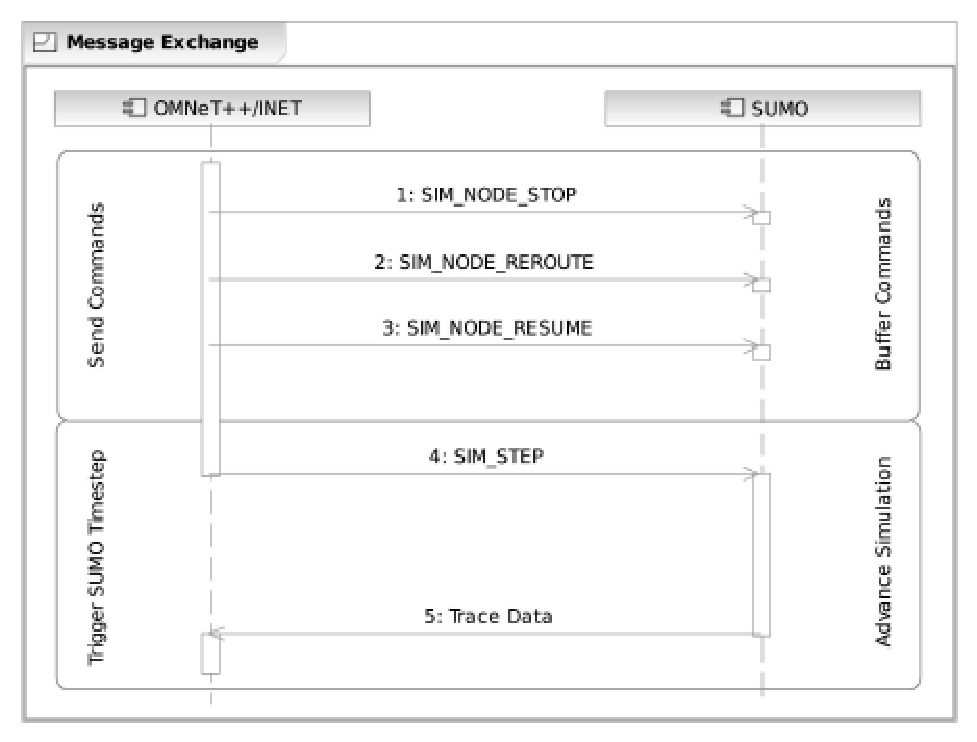
\includegraphics[width=0.8\textwidth]{img/bidirectional_com}
\end{figure}

Messages may contain any sort of data, in addition to usual attributes such as
timestamp. They are sent via gates, the in and out interfaces of modules.
Connections are created within a single level of module hierarchy, they are not
possible across multiple modules as they would obstruct model reuse. Because the
hierarchical structure of the model, messages typically travel through a chain
of connections.

Given the type of network we need in our implementation, we use an
open-source framework for running vehicular network simulations called Veins \cite{veins}.
It uses Simulation of Urban Mobility (SUMO) along with Omnet++, connected
through TCP sockets, to perform Inter-Vehicular Communication evaluations.

Simulation of Urban Mobility (SUMO) is a microscopic road traffic simulation
package designed to handle large road network \cite{sumo}. Thus, we can perform
bidirectionally-coupled simulation of road traffic and network traffic. Movement
of nodes in Omnet++ simulation is determined by movement of vehicles in road
traffic simulator SUMO. Nodes can then interact with the running road traffic
simulation.

\section{Network Description in Omnet++}

The user must describe the structure of the simulation model in a language
called NED. NED stands for Network Description and allows the user to declare
simple modules, and connect and assemble them into compound modules. It has
several features which let it scale well to large projects.

\begin{itemize}
  \item Hierarchical. Any module which appears to be complicated, can be
  split into smaller modules, and used as a compound module.
  \item Component-Based. It provides module reusability, reducing code
  copying, and more importantly allows component libraries like Veins to exist.
  \item Interfaces have a special purpose: they replace a module or channel type
  that would normally be declared in the network description. The concrete
  module or channel type is determined at network setup time by a parameter.
  Concrete modules types must implement the interface they substitute. For
  example, a compound module type named MobileHost contains a mobility submodule
  of the type IMobility (an interface); the actual type of mobility may be
  chosen from the module types that implemented IMobility (RandomWalkMobility,
  TurtleMobility, etc.)
  \item Inheritance. Modules and channels can be inherited like C++ classes.
  Extended modules could add new parameters, gates, new submodules
  or connections. They may initialize some parameters to default values.
  \item Packages. The NED language has a package structure similar to Java
  language. Its main purpose is avoid name conflicts between different modules.
  It has a similar ``CLASSPATH'' called NEDPATH introduced to make it easier to
  specify dependencies among simulation modules.
\end{itemize}

\section{Architecture}
Every simulation in Omnet++ is defined by a configuration file, usually called
\mbox{\it omnetpp.ini}. It contains settings that control how the simulation is
executed, values for model parameters, etc.

\subsection{Network}
The most important parameter which has to be defined in the configuration file
is the network module type (if it is not defined in the configuration file it
will be asked for at runtime). Our network is called simply FloatingScenario and
extends a simple module called FloatingContent. Networks usually consist
of two main important section: first include the nodes that form the network,
and second include how the nodes are to be connected. In our particular case the
nodes are vehicles which are moving across a map, so they are not static and its
defined based on multiple files (we will talk about it later in the document).
The module which handles this information is TraCIScenarioManagerLaunchd.

It contains the next submodules:

\begin{itemize}
  \item ObstacleControl model uses obstacles from poly file resulted from the
  map export in order to block the radio transmission as in real world. The
  obstacles refer mainly to buildings which exist on the map, and may block
  radio propagation of signals between vehicles.
  \item AnnotationManager manages annotations in Omnet++ canvas. It displays
  module graphical representation (as icon) or additional representation
  strings.
  \item ConnectionManager handles all connection related stuff. It will be
  discussed in detail later in the document.
  \item WorldUtility extends basic module BaseWorldUtility which provide utility
  methods and information used by the whole network as well as simulation wide
  black board functionality. It collects global parameters like the dimensions
  of the network (playground), whether is 2D or 3D, anchor range and distance
  between them.
  \item TraCIScenarioManagerLaunchd extends TraCIScenarioManager and handles
  nodes from the network details.
\end{itemize}


\subsection{Traffic Simulation}

Traffic simulation in {\it Veins} is done with the help of microscopic road
traffic simulation package SUMO. It can perform simulations both running with
and without GUI and it is able to import city maps from a variety of file
formats including OpenStreetMap types.

SUMO deals with high-performance simulations of huge networks with roads
consisting of multiple lanes. Vehicles can move accordingly to a configured
timetable, dynamically generated routes, or statically assigned routes
\cite{veins}.

The connection between SUMO and Omnet++ is done with the help of TraCI: Traffic
Control Interface. Is an architecture that couples two simulators: a road
traffic and network simulator. It is important to know that mobility patterns
are not pre-defined as fixed trace files. The traffic and network simulators are
connected in real time, enabling the control of mobility attributes of each
simulated vehicle. The reason there are no predefined routes is the fact that
the mobility of each car can be influenced by the network simulator, based on
the information it receives (for example a bad weather warning).

We denote {\it TraCI-Server} the road simulator and the {\it TraCI-Client} the
network simulator. They are connected over a TCP connection for exchanging
messages. So when the connection is established, the network controls the
traffic simulator via the data exchange protocol, enhancing the control of the
movement for each vehicle. Data exchanges are controlled by the client that
send commands as requests to the traffic simulator. The traffic simulator
may respond to each command once or multiple times.

Time synchronization between both simulators is performed by the client which
sends periodically, at each simulation step, e.g. 1[s], a message to the road
traffic simulator that contains the current simulation time plus one simulation
step. The road traffic simulator computes the next step and sends the data to
the network simulator. The vehicle positions are converted into linear movements
by the network simulator, in order to allow all vehicles to reach their
positions at the time specified by traffic simulator. The execution of the
atomic mobility commands is delayed by one simulation step, because the road
traffic simulator is always one simulation step ahead. This may represent a
drawback of the method, but considering the very short simulation time step -
for traffic efficiency applications approximately 1[s] and for safety
applications - 0.1[s], the drawback is negligible. When the network simulator or
road traffic simulator ends, it closes the TCP connection, and causes the other
simulator to stop immediately \cite{traci_interface}.

TraCIScenarioManagerLaunchd is the manager module which handles the Traffic
Control Interface. Parameters $host$ and $port$ indicate Omnet++ the address and
the port on which SUMO listens for connections. We can specify the time interval
of host's position updates by setting $updateInterval$. Parameter $moduleType$
specifies the module type to be used in the simulation for each managed vehicle.

\subsection{Connection modeling}

Connectivity modelling is a more difficult task to be designed in wireless
networks than in the wired one. In the latter case, connectivity is achieved with wires
which in Omnet++ are easily modelled with $connections$. The channel between two
nodes in a wireless network is basically the air and cannot be represented just
by one connection, because is a broadcast medium. $ConnectionManager$ module
manages the connectivity in our simulation.

In theory, signals sent out by a node may affect all other node in the
simulation. Adding attenuation makes the power of the signal very low for the
nodes which are far away from the origin, and thus making it negligible.

As presented in \cite{Kopke}, the $maximal interference distance$ is a
conservative bound on the maximal distance at which a node can still disturb the
communication of a neighbour. In order to reduce the computational complexity,
MIXIM connects nodes only if they are within the maximal interference distance.

The objects present in the propagation environment influence the $maximal
interference distance$ by reducing it due to the additional attenuation they
imply. It may cause disconnection between two nodes, leading to the hidden node
problem.

It is important for safety applications to perform IVC simulations as realistic
and correct as possible. Thus, a model for modeling buildings and their
properties must be used, to accurately simulate the signal propagation. One
type of building generated attenuation is shadowing, defined as the fluctuations
in received signal power. In ~\cite{sommer2011computationally} is presented a
realistic and computationally inexpensive simulation model for IEEE 802.11p
radio shadowing in urban environments. It is validated using real world
measurements in a city scenario for different types of obstacles. The obstacle
model is integrated in the Veins making it suitable for our simulation needs.

In Omnet++ gates are the connection points of modules. There are three types of
gates: $input$, $output$, $inout$, the latter having the behaviour of the first
ones. Gates can only be connected to other gates via $connections$. These
$connections$ are found in the network description files (NED) of the modules.

Every node module registers its network interface card (nic) to the
$ConnectionManager$ along with its position. Every time the node position
changes, the manager is notified, and after the calculations taking into
consideration the new value and the attenuation, it updates the list of
neighbours which the node can establish connections with.

$Nic$s have an $input$ $connection$ called $radioIn$ which expects messages from
other modules. So whenever a node sends out a message, the $ConnectionManager$
passes it to the list of neighbours computed as we mentioned above, using
$sendDirect()$ function. The function receives the module and the gate id as
parameters. The neighbours pass the received message further to the upper
layers.

\begin{figure}[bt]
 \centering
 \begin{subfigure}[b]{5cm}
 	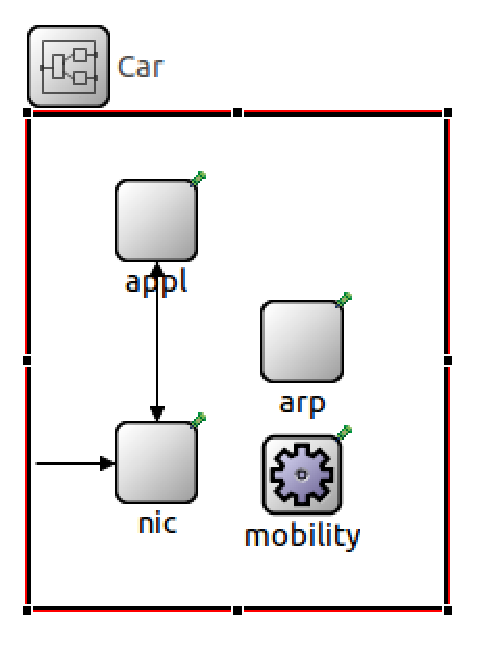
\includegraphics[width=5cm]{img/CarNode}
 	\caption{Car module}
 	\label{fig:car}
 \end{subfigure}
 \begin{subfigure}[b]{5cm}
 	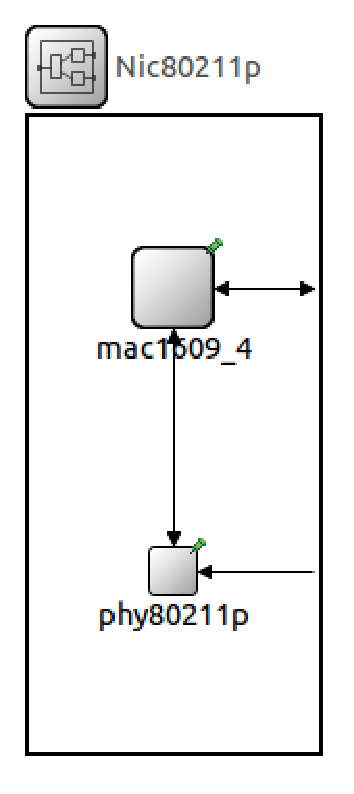
\includegraphics[width=3cm]{img/Nic80211p}
 	\caption{Nic module}%
 	\label{fig:nic}
 \end{subfigure}
 \caption{Car and Nic modules}
 \label{fig:car_nic}
\end{figure}

\section{Car modules}
Nodes in Omnet++ network are entities desiring to communicate with each other.
The Car node module, we are using in our simulation, can be seen in
~\ref{fig:car}. In the left side appears the standard layer according to WAVE
protocol, the application layer (appl), the MAC layer and the physical
layer (phy). The physical layer takes care of the reception and collision
handling. Layers are modules connected by two pairs of Omnet++ ``gates''. The
first one is used for transferring data up and down as in the real world
protocol stacks, the second one is for exchanging messages between the layers
and support the control communication, e.g. a request from the MAC layer for PHY
layer to perform carrier sensing, or notification of PHY layer that the
transmission of data is over.

The MAC and physical layer are grouped into a module called Network Interface
Card (NIC) in Figure ~\ref{fig:nic}, because they their design is usually
tightly coupled and specific for different communication techniques like
bluetooth or GSM. A node can have multiple different NICs.

The mobility module performs movement of a node or object. It will be discussed
in a further section. The arp module runs the Address Resolution Protocol which
translates the network address into a MAC address. The application module is the
top layer and uses the network interface card to send messages. It is the
application equivalent in the IP stack.

\subsection{Car mobility}

In our simulation, we use TraCIMobility module which extends BaseMobility and
relies on TraCIScenarioManager for state updates. Basically, the
TraCIScenarioManager holds a list of nodes updated continuously from the road
traffic simulation through the TCP connection. Every simulation step, determined
by the $updateInterval$, the module iterates over the entire node list, reads
the next node position on the road and updates the fields accordingly.

The BaseMobility class takes care of the graphical representation of the module.
So every change of the position is reflected into the on the graphical
representation. It publishes the new position so that other modules get
informed, e.g the physical layer must update the position with the
ConnectionManager. It also takes care of exiting the border.

TraCIMobility contains a field called $statistics$ which records generated data
during the simulation. Recorded information are: $startTime$, $stopTime$,
$totalTime$, $totalDistance$, $minSpeed$, $maxSpeed$ and much more could be
added.

\subsection{WAVE: Wireless Access in Vehicular Environment}

WAVE is system architecture built by IEEE and its main objective is to
facilitate communication between vehicles and road side infrastructure. The
reason why other existing standards aren't used is because they don't work
efficiently with authentication and update of routing tables with the continuous
changing network topology and short amount of time available for connection and
communication.

Our NIC module implements an 802.11p interface card, with the physical and
medium access control layers based on the IEEE standard, because it is a widely
known standard with many manufacturers guaranteeing interoperability. Some
features of 802.11p standard are \cite{phule2012public}:
 
\begin{itemize}
  \item {\it Fast connection setup} is a necessary behaviour when running in a
  highly dynamic network topology, because the time spent in the communication
  range of other node is very short. For example the case of two vehicles
  travelling in opposite directions, on a high speed highway.
  \item {\it Random MAC address} ensure the anonymity of the vehicles make them
  untraceable. It makes it difficult to associate data, collected over the
  ad-hoc network, with a specific node and track it using this data.
  \item {\it Priority Control} helps achieve Quality of Service (QoS) in the
  applications running over the ad-hoc network. It prioritizes data from
  different applications and provides critical data access to the channel.
  \item{\it Power Control} enables the applications to specify the transmit
  power used to pass each packet over the channel. Customizing this from the
  application is useful, because one can modify it according to the surrounding
  topographical characteristics.
\end{itemize}



\subsection{Physical layer}

As \cite{Kopke} presents, the physical layer is the core of the wireless node in
MIXIM framework. It provides message sending and receiving, collision detection
and bit error calculation.

The MIXIM physical layer has three components described in details: the
BasePhyLayer which provides the interfaces to the MAC layer, the AnalogueModel
which is responsible for simulating the attenuation of received signal and the
Decider responsible for evaluation and demodulation of the received messages.
The analogue and decider modules are pure C++ classes.

The signal strength is influenced by the environment it travels in order to
reach the destination node. It can be modeled with attenuation factors caused by
path loss, shadowing and fading, and can be sent with multiple frequencies.
Thus, a message can have varying sending power, attenuation, and bit-rate in
time, space and frequency. MIXIM attaches to every message a signal object
representing sending power, attenuation, and bit-rate in three dimensions time,
frequency and space. The receiving node adds the attenuation.

When the physical layer receives a message, it passes the message to the
analogue model to compute the attenuation part of the signal. It is
also responsible for simulating the propagation and transmission delay of the
message. The message is passed at least twice to the decider, at the beginning
and the end of it transmission. The decider can request the message any time
in-between. After the decider calculates the bit errors, the message reaches the
MAC layer. The BasePhyLayer acts as an interface between physical layer
messages(AirFrame) and the AnalogueModel and the Decider. The physical layer
stores all messages in the ChannelInfo class which can compute the AirFrames
intersecting with a given time interval. This is useful for the decider that
calculates the signal-to-noise ratio (SNR) of a given message.

MIXIM simulates path loss, shadowing and fading, because Omnet++ doesn't have
attenuation. The physical layer supports multiple analogue models, each one
representing basically a filter class for signals. Summing up the attenuation
from all analogue models, gives the attenuation part of the signal, calculated
at the beginning and at the end of the message reception. The decider can
calculate then, together with the sending power of the received message, the SNR
and the bit errors.

The Decider is responsible with performing three main tasks: must classify
incoming messages into noise or valid messages, must calculate the bit errors
for a valid message when its reception is over and must provide information
about the current state of the channel.

When the physical layer receives a message, it is sent to the decider which can
either decide immediately whether the message is noise or not, or it can force
the physical layer to resubmit the packet after a certain amount of time. This
enable the decider to revise its decision, if a second stronger message arrives
in the mean time.

The decider can request the message from the physical layer the latest at the
end of message reception process. This moment is also the time for the decider
to compute the bit errors for the message. It uses all the intersecting
messages from the ChannelInfo in order to calculate the SNR. Then it can
calculate bit errors and positions depending on the complexity of the particular
decider model.

In the end, the decider must provide information about the channel state, needed
at the MAC layer for Carrier Sense Multiple Access (CSMA) protocols. The MAC
layer can request the decider to check the channel and return if it is currently
idle or busy.

\subsection{MAC layer}

The Medium Access Control (MAC) protocol has the purpose to handle the medium
for communication between nodes in the system. Since we use a wireless system
the air represents the shared medium. Thus, the protocol needs to decide the
moment when a node should emit signals in order to transmit a message, to avoid
interference with signals from other nodes.

The IEEE 1609.4 standard is used which support the following features as shown
in \cite{phule2012public}:

\begin{itemize}
  \item {\it Control Channel Monitoring} : nodes have to monitor the channel at
  a predefined interval.
  \item {\it Synchronized Switching}: devices with a single channel cannot
  monitor the Control Channel and the Service Channel at the same time. Thus,
  they must synchronize to monitor the Control Channel at the same time, to be
  able to communicate.
  \item {\it Channel Routing} passes the data from the higher layers to the
  right channel. It also passes the data from the low layer to the correct
  networking protocol.
\end{itemize}

The model is discussed in detail in \cite{eckhoff2012multi} and the
implementation is available free and open source for Omnet++ simulator included
in Veins framework for IVC simulation.

\begin{figure}
	\centering
	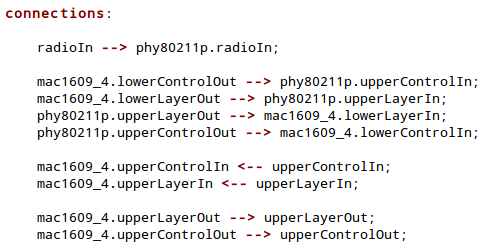
\includegraphics[width=0.6\textwidth]{img/nic80211p_connections}
	\caption{Connections between physical and MAC layers.}
	\label{fig:nic80211p_connections}
\end{figure}
 
Figure \ref{fig:nic80211p_connections} displays the $connections$ between
the physical module and the MAC module. This section states that all messages
from the physical module are passed through the $upperLayerOut$ gate and they
are received at the $lowerLayerIn$ gate of MAC layer. Analogue connections exist
when messages come from the upper layers. The $radioIn$ ensures all messages
received are sent to the physical module to simulate the their reception. In
fact messages come from $ConnectionManager$ as we stated above.

\begin{figure}[t]
	\centering
	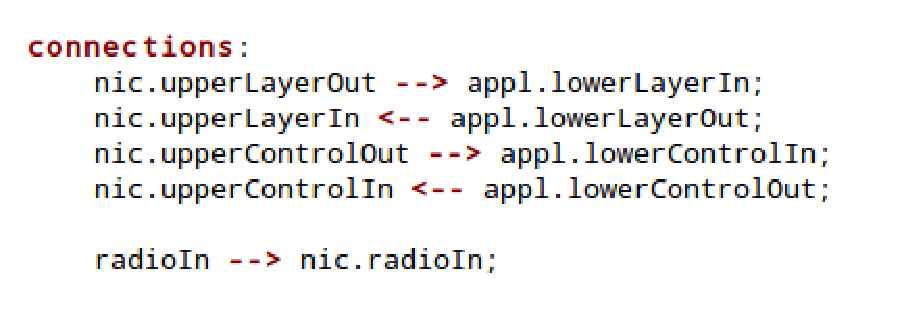
\includegraphics[width=0.6\textwidth]{img/appl_connections}
	\caption{Connections between newtork interface card and application
	layer.}
	\label{fig:appl_connections}
\end{figure}

\subsection{Application layer}

The application layer runs the algorithm which handles the exchange of the
messages between the nodes and is the top layer in the IEEE802.11p standard. Our
application module is called FloatingContentApp and extends BaseWaveApplLayer.
Figure ~\ref{fig:appl_connections} shows the pair of connections between the two
layers.

The most useful feature our application inherits from the BaseWaveApplLayer is
the beaconing system, used in our application for peer discovering. In Omnet++
scheduling future events in order to implement timers, timeouts or delays is
performed by letting the simple module to send a message to itself. The messages
are called $self-messages$ and are delivered later to the simple module. It does
not use the network interface card for its implementation. Self-messages are
sent using $scheduleAt()$ function which accepts absolute simulation time and a
type of message for event identification as parameters. They are sent as regular
messages and can be identified by using $isSelfMessage()$. We use self-messages
to schedule beacons at an interval of 300s, a value which is read from the
configuration file.

Regular messages are sent down to the lower layer using $sendDelayed()$ which
keeps the message for a delay interval and send it afterwards. The message,
delay value and gate id are the method arguments.

Messages arrived at a module are handled in $handleMessage()$ method where a the
application can decide to which callback to pass it based on the gate it arrived
on. This method is specific to $BaseLayer$, a class extended by
$BaseWaveApplLayer$ which call $handleSelfMessages()$ for $self-messages$,
$handleUpperMsg()$ for messages from upper layers and $handleLowerMsg()$ for
messages from the lower layers. $BaseWaveApplLayer$ classifies again the
messages received in $handleLowerMsg()$ in ``beacons'' or ``data'' and call the
methods implemented by FloatingContentApp, $onData()$ and $onBeacon()$, accordingly.

Since our application must be aware of the node localization, there must be a
method to send notifications from the road traffic simulator towards the network
simulation at every simulation step. As we presented in an earlier section, the
TraCIScenarioManager which handles message exchanges between the two simulators,
updates the positions for every mobility module specific to a vehicle. Every
mobility must notify the application module about the new position. Omnet++ has
implemented a publish-subscribe style communication among modules. The advantage
is that the two communication modules might not know about each other and
possibly there is many-to-many relationship among them. In our implementation,
the two modules we talk about are the $mobility$ module and the $application$
module.

Thus, every position update the network simulator receives, reaches the
traffic scenario manager which notifies every mobility module in the network.
The mobility module then signals the application module with a signal called
$mobilityStateChangedSignal$ and with the help of $emit()$ function. The function
takes the mobility module as argument to pass the new position in the
application module.

The application must subscribe to the mobility state change signal in order
to start listening for these type of events. The listeners use $receiveSignal()$
function to handle the received signals and decide next steps according to their
type. In our case the callback function $handlePositionUpdate()$ is called, which
computes results with the new position.

When a node appears in the simulation the $initialize()$ method of each module
and its submodule is called to perform data initialization. The application's
ancestor class, $BaseWaveApplLayer$ schedules the discovering system based on
beacon messages.

We stored into a vector container the coordinates of the anchor zones we
received information for. Thus, when a peer is discovered i.e. a beacon is
received, we encapsulate the list into a wave short message and send it out to
the sender of the beacon. Since the message is broadcasted, we simulate
unicasting by checking that the message recipient address field is the same with
the current node id. Otherwise we discard the message.

\section {Collecting Simulation Data}

Omnet++ has built-in support for recording simulation data, via output vectors
and output scalars. Output vectors give the full picture of what is happening
during the simulation, while the output scalars are summary results, computed
during the simulation and written out when the simulation completes. We use the
latter in our simulation in order to compute the $criticality$ condition.

To estimate the feasibility of floating content, we positioned anchor zones
every 200m in a grid across the simulation area as shown in the figure
~\ref{fig:SanFrancisco_Anchors}. More details about the simulation environment
in the next chapter.

Every anchor zone has its own independent module which records multiple
statistics during the simulation : the total number of vehicles crossing the
anchor, the average sojourn time of a vehicle, the number of contacts of a
vehicle during its sojourn time, etc. We decided to hold this data inside the
$TraCIScenarioManager$ module due to its importance and the fact that it is
unique and provides the same data to all the modules.

With the help of $handlePositionUpdate()$, we can track the vehicles inside an
anchor zone. We use different replication ranges for the anchor zones which are
bigger than the distance between them. This results in having overlapped anchor
zones. Determining all the anchor zones a vehicle resides in, may be quite a
challenge.

Our approach is very simple and complexity optimised. Based on the position of
the vehicle, the box in which the vehicle resides from the grid can be
determined. Each of the corners represents the center of an anchor zone. If the
radius of an anchor zone is equal with the distance between the anchor zones,
the vehicle can reside in some or all the anchor zones placed in the corners of
its box as shown in Figure ~\ref{fig:node_az}. If the radius is bigger, than we
process all the anchor zones that are farther and contain the vehicle.
Opposed to iterating over all anchor zones and perform operations, this method
reduces the computational complexity.

\begin{figure}[t]
	\centering
	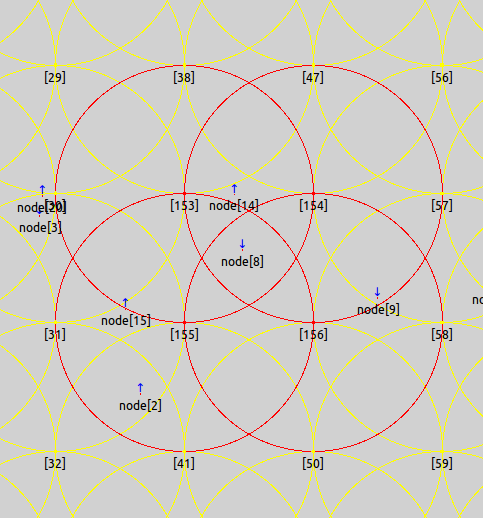
\includegraphics[width=0.4\textwidth]{img/node_az}
	\caption{Anchor zones in which node number 8 resides, are coloured with red,
	the other ones are coloured with yellow.}
	\label{fig:node_az}
\end{figure}

When an encounter takes place i.e. a module receives a message and $onData()$
method is called we must check if both nodes reside in the same anchor zone as
the calculation of $criticality\ condition$ requires. Thus, we keep the above
algorithm for anchor zones calculation, but we verify if both vehicles, the
sender or the receiver reside in the same anchor zone.

The following values are recorded and calculated in our simulation :
\begin{itemize}
	\item {\it maxTransitNodes} represents the maximum number of nodes that exists
	at a given time in the anchor zone.
	\item {\it avgContactsInSJNTime} represents the average number of contacts in
	their sojourn time.
	\item {\it avgTimeInAnchor} denotes the average sojourn time of vehicles in an
	anchor zone.
	\item {\it criticality} which is equal to $maxTransitNodes$ *
	$avgContactsInSJNTime$ * $avgTimeInAnchor$.
\end{itemize}

% ==== Simulation Environment and evaluation (CHAPTER 4) ================================================

\chapter{Simulation Environment and Evaluation}

In this section we will discuss about the simulation environment, traffic
generation and the evaluation of resulted data.

\section{Environment}

The environment for our simulation required by Omnet++ was generated using
OpenStreetMap ~\cite{openstreetmap} and several SUMO tools. We decided to use
three different city scenarios to show that floating content in urban
environments can be feasible regardless of particularity of road
architecture. The cities we used as simulation environment are: SanFrancisco,
Beijing and Berlin.

The road network file is generated from the exported map (from OpenStreetMap)
file using $netconvert$. It has many paramaters that steer how the network is
imported and how the resulting SUMO-network is generated. We removed
isolated edges because they have no influence and benefit for the simulation
scenario. We also removed the unnecessary nodes that split edges without being
at a junction. We clustered junctions with traffic lights and joined the traffic
light logic.

OpenStreetMap contains not only the road network, but also a wide range of
additional polygons such as buildings and rivers. They represent the obstacles
existing on the map which generate signal attenuation and influence the
communication between vehicles.

As suggested in \cite{percomfloatingcontent}, we also chose two different anchor
zone radii: $a$ = $r$ $\epsilon$ \{200m, 500m\}. To evaluate the feasibility of
floating content in the urban area we placed anchor zones every 200m
horizontally and vertically across the entire simulation area. Figure
~\ref{fig:anchor_zones_grid} shows how anchor zones are distributed on the
simulation map.

\begin{figure}[t]
 \centering
 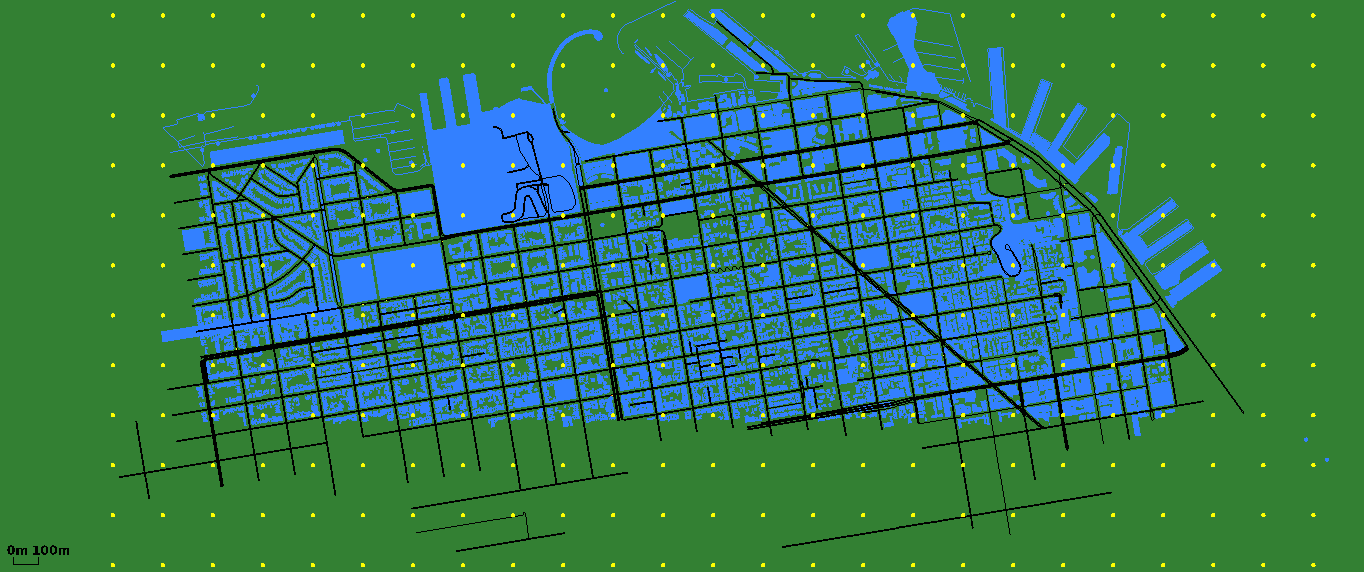
\includegraphics[width=15cm,height=14cm,keepaspectratio]{img/SanFrancisco_Anchors}
 \caption{Anchor zones every 200m over the simulation area}
 \label{fig:anchor_zones_grid}
\end{figure}

\section{Mobility Simulation}

There are many methods used to obtain suitable mobility pattern for simulations
in urban vehicular scenarios. In this section we briefly describe several
relevant mobility patterns.

One of the most popular mobility models to evaluate mobile ad hoc network
(MANET) routing protocols is called ``Random Waypoint Model''. It became popular
due to its simplicity and wide availability. Each node following this mobility
pattern pauses for a fixed number of seconds and selects a random destination
in the simulation area and a random speed between 0 and some maximum speed. When
it arrives at the destination it repeats the previous step. Despite of its
simplicity, the analysis from ~\cite{yoon2003random} revealed that it can be
harmful when simulating vehicular ad hoc networks.

Real mobility traces is another method to obtain mobility models and presents a
clear improvement over the random mobility. Traces are obtained from real
vehicles such as taxis and buses which simply move in an ordinary day in a city.
The mobility of nodes is tracked using on board equipment or road side
equipment. Although they generate the most realistic mobility patterns, it is
clear that it is influenced by other non tracked vehicles whose movement does
not appear in the recorded traces. The major problem is that it lacks
flexibility and does not allow performing exhaustive evaluation of ad hoc
network protocols. For example we cannot change vehicle density without
modifying speed ~\cite{baguena2013vacamobil}.

As we stated in the previous chapter we use the SUMO road traffic simulator
which overcome the restrictions of real traces with no loss of realism. SUMO
defines two concepts used to generate traffic for a map generated network: trips
which denotes the origin and the destination for a single vehicle, and flows
which defines the same trip for multiple vehicles. We used a couple of SUMO
tools to generate our traffic demand:

\begin{itemize}
  \item {\it randomTrips.py} is a random trip generator. It inserts a
  new vehicle every second with a trip having a random origin and destination.
  It doesn't check if the two locations on the map are connected.
  \item {\it duarouter} generates the traffic demand using a file with trips and
  flows. It is made up of vehicles with assigned routes, calculated using the
  Dijkstra algorithm. Unconnected trips are deleted.
\end{itemize}

We ensured that every car travels a minimum distance of 1500 meters from origin
to destination. $randomTrips.py$ distribute the vehicles randomly on their
starting edges taking into account their speed and the edge maximum speed. We
decided to place a bigger proportion of high speed vehicles on the map which
will be placed on lanes with higher maximum speeds. This way, there will
be heavy traffic on highways and anchor zones with higher $criticality\ 
conditions$ should appear in the areas where the traffic jams may occur. It is a
method to emphasize the anchor zones with high floating probability without loss of
generality. The speed ranges from ~5m/s ( ~18km/h ) to ( ~79km/h ).

\section{Evaluation}

We decided to perform simulations using different time values, to observe the
behaviour of $criticality\ condition$: $t\ \epsilon\ \{300s, 600s\}$. Although
time intervals appear to be short, they are sufficient for gathering consistent
data. Since the application relies on data broadcasting, it forces the simulator
to schedule thousands of messages which results in usage of a great amount of
time and memory. For example, 10 minutes of simulation for San Francisco city
was processed in 1 hour and 45 minutes.

\subsection{Beijing}

Figure ~\ref{fig:Beijing_300s} depicts the value of the $criticality$ for each
anchor zone. Figure ~\ref{fig:Beijing_waiting} is a snapshot that displays the
road network from an area of 6.7$\times$5.2 km$^2$. The map is coloured with
respect to the amount of time a car has to wait due to the traffic lights placed
in intersection. Road segments coloured in red have a bigger waiting time than
the one coloured in black.
  

\begin{figure}[t]
\centering
	\begin{subfigure}[t]{1\textwidth}
	\centering
	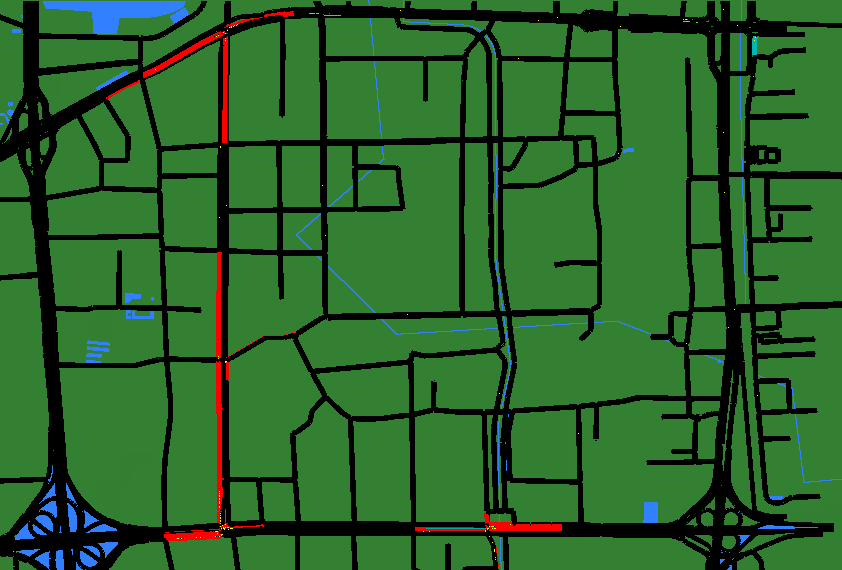
\includegraphics[width=0.8\textwidth,height=6cm]{img/Beijing/Beijing4}
	\caption{Beijing traffic waiting time heatmap}
	\label{fig:Beijing_waiting}
	\end{subfigure}
	
	\begin{subfigure}[t]{0.5\textwidth}
 		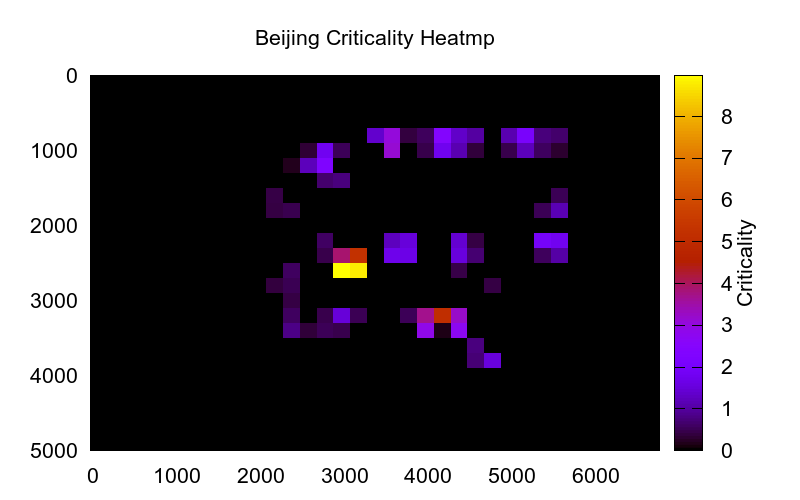
\includegraphics[width=\textwidth]{img/Beijing/criticality3_sim_Beijing3_300s_200m}
 		\caption{Beijing Criticality Map $r\ =\ 200m$}
 		\label{fig:Beijing_criticality_300s}
 	\end{subfigure}%
 	\hfill
 	\begin{subfigure}[t]{0.5\textwidth}
 		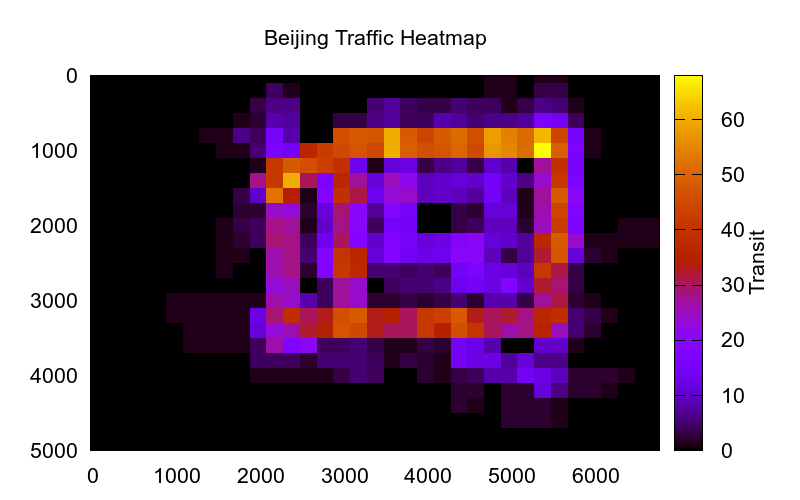
\includegraphics[width=\textwidth]{img/Beijing/transit_sim_Beijing3_300s_200m}
 		\caption{Transit Map $r\ =\ 200m$}
 		\label{fig:Beijing_transit_300s}
 	\end{subfigure}
 	
 	\begin{subfigure}[t]{0.5\textwidth}
 		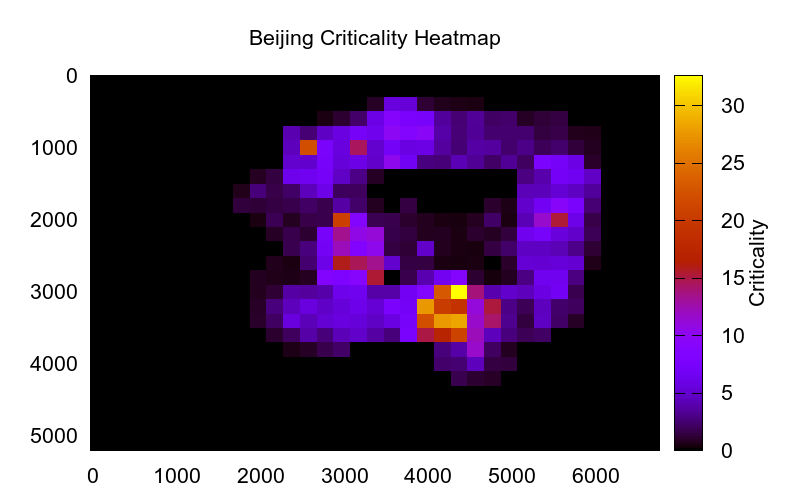
\includegraphics[width=\textwidth]{img/Beijing/criticality3_sim_Beijing3_300s_500m}
 		\caption{Beijing Criticality Map $r\ =\ 500m$}
 		\label{fig:Beijing_criticality_300s}
 	\end{subfigure}%
 	\hfill
 	\begin{subfigure}[t]{0.5\textwidth}
 		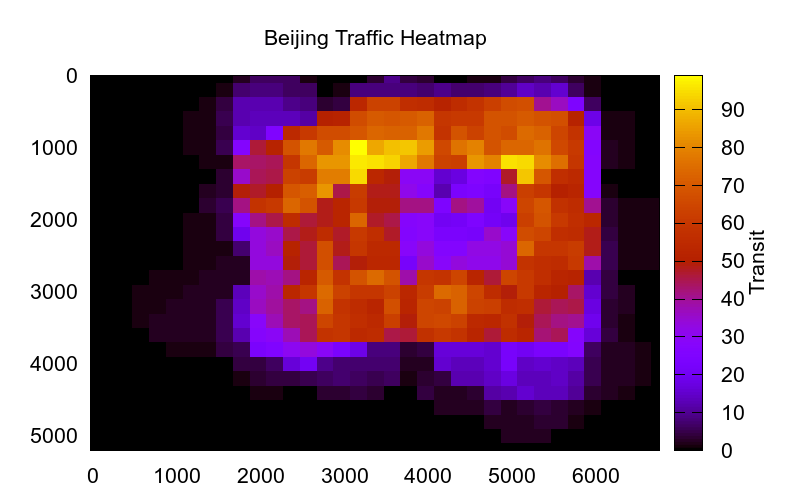
\includegraphics[width=\textwidth]{img/Beijing/transit_sim_Beijing3_300s_500m}
 		\caption{Transit Map $r\ =\ 500m$}
 		\label{fig:Beijing_transit_300s}
 	\end{subfigure}
 	\caption{Beijing 300s simulation}
 	\label{fig:Beijing_300s}
\end{figure}
